% !TEX root = ../../thesis.tex

% Photo Yves Gellie
% 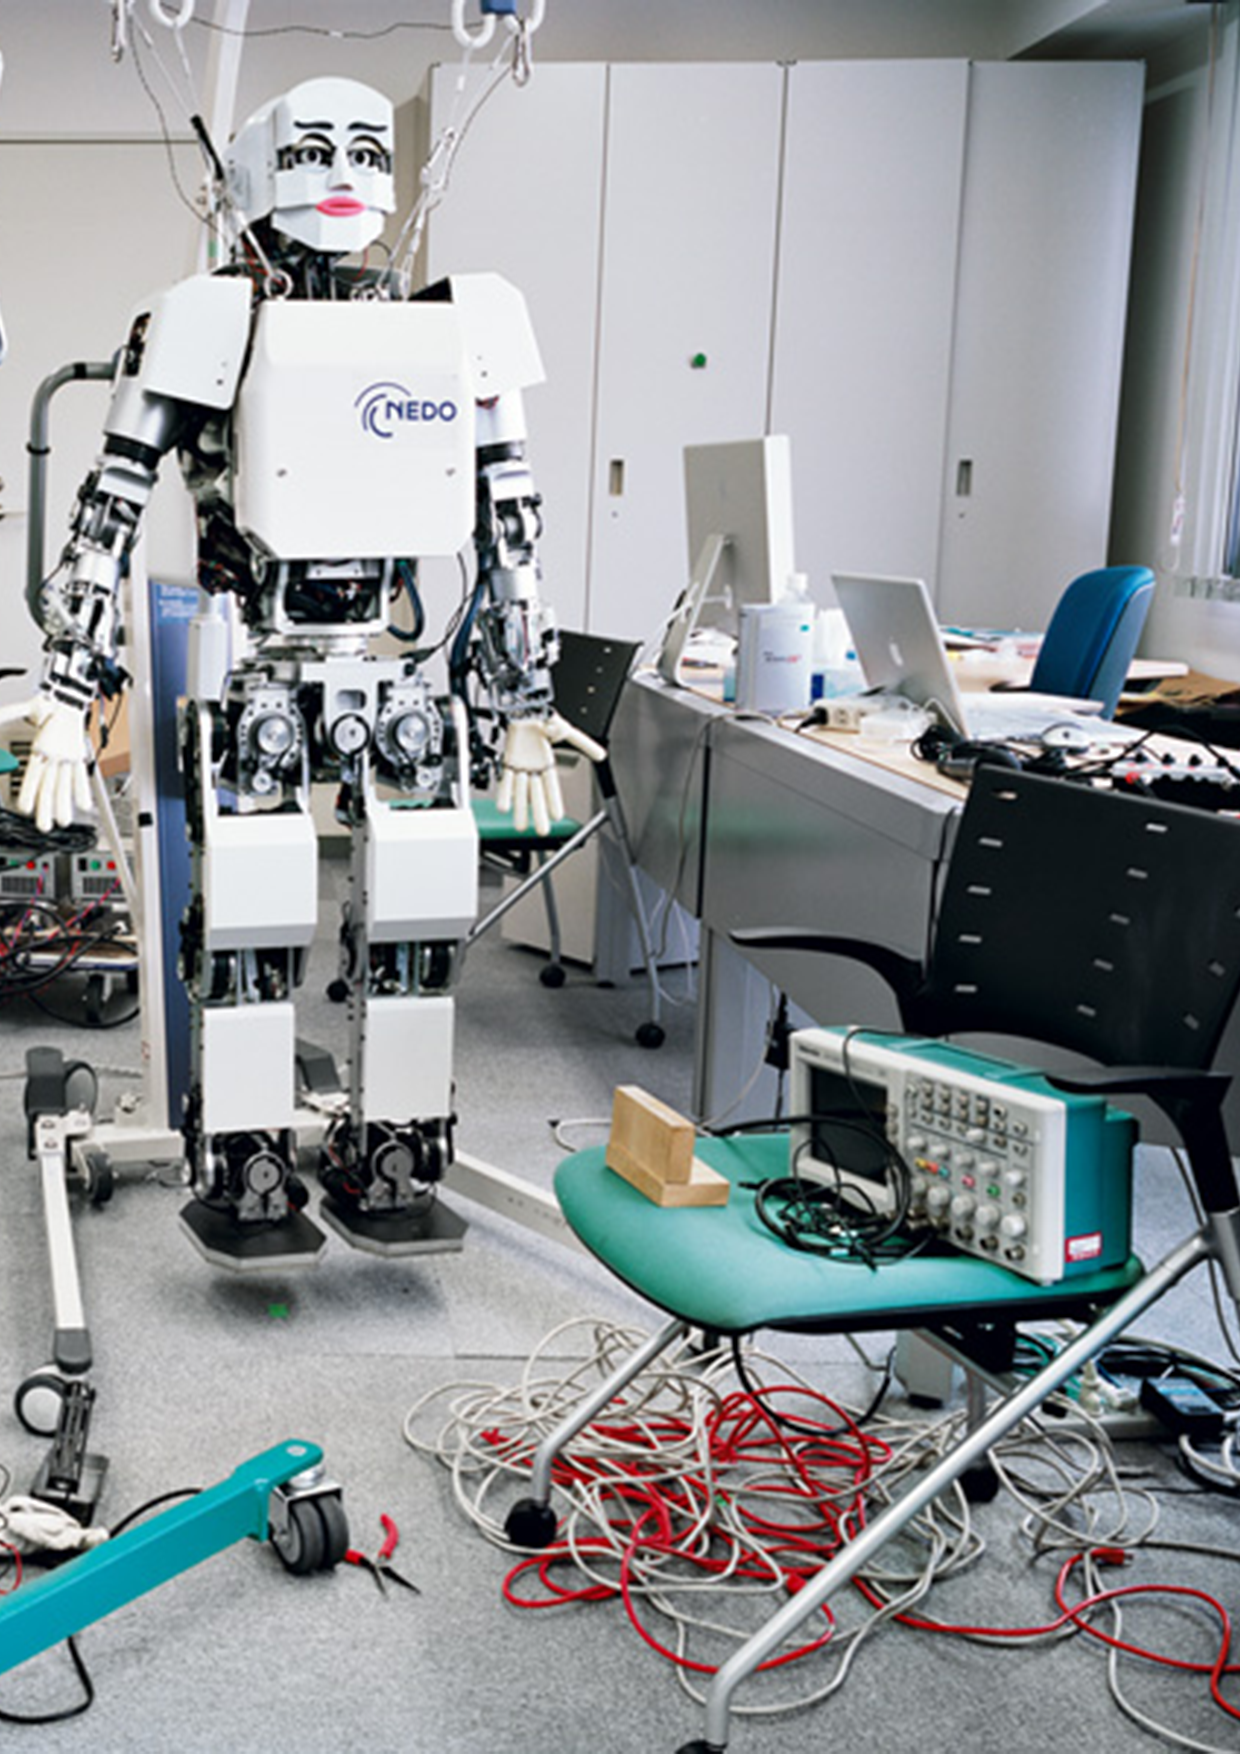
\includepdf{/Users/matthieulapeyre/Documents/phd_thesis/media/robot_setup.pdf}
\chapter{Review of experimental methods} % (fold)
\cleanchapterquote{The world is its own best model}{Rodney Brooks}


\section{Introduction} % (fold)

As we saw it in the previous chapter REF, an interesting evolution of the last decades is the demonstration of the importance of the morphology for sensorimotor control, cognition and development. The role of the morphology appears as a fascinating open field. Exploring the interaction between body properties and cognition could lead to both a better understanding of animals’ behaviour (human being in particular) and to build robot more adapted and robust to an open environment with unpredictable interaction.

However as Rodney Brooks explained, exploring interaction between morphology, cognition and environnement requires real world experimentations. Indeed embodiement artificial intelligence REF needs to act in the real world to permit the emergence of complex behavior. The real world includes a large amount of constraints such as inertia, multi-point physical contacts, unpredictable environnement or friction which are, at this time, too complicated to be modeled in physical simulator. Actually "The world is its own best model" and if we can use simulation for exploring basic concepts, the exploration of emergent complex behavior based on interaction between robot self-dynamics and the environnement can only be done through experimentation with real robot in real world.


A great example of achieving complex behavior using robot dynamics is the passive walking (see REF). One of the best sate of the art in this domain is the work done by Delft with the different passive and semi passive walkers they built.

Desiring to explore biped locomotion with Poppy, I had a discussion with Martijn Wisse on simulation strategy to add semi-passive abilities to Poppy. Here is his answer:

\begin{quotation}
First of all, we never actually produced a high-fidelity simulation. We made very simple simulations only. From them, we learned how to tune parameters. Then, we designed the real robots, without running full-blown optimizations. Rather, we used our intuition for a large number of decisions on design trade-offs, using lessons from the simple simulations combined with other limitations such as available motors etcetera. Then, we (again) used our intuition and large amount of experience to tune the robot’s controllers, and make design improvements, until it walked.

\signed{Martijn Wisse - Associate professor at Delft University of Technology}
\end{quotation}

But maybe the most interesting part concerns the work they did to try to make their robot walk in simulation:

\begin{quotation}

Even after obtaining a successful walking motion, we did not manage to create a simulation that walked successfully using the same controller parameters. We tried very hard with some of the best people, but we didn’t succeed. The reason was, I think, that our type of control (using the emergent behavior of a set of simple reflex-like controllers) was highly sensitive to hardware effects like friction. Normally, one uses a local joint controller to make the joint follow a desired trajectory independent of the exact amount of friction. The local controller “abstracts these hardware effects away”, if you know what I mean. This makes the behavior of the whole system quite predictable. However, in our robots, we did not have this kind of abstraction as we were not following trajectories, and thus a little bit of extra friction has an effect on the entire motion.

We did spend a long time making a high-fidelity model in Adams, and also using other methods, but eventually we gave up without success.

\signed{Martijn Wisse - Associate professor at Delft University of Technology}
\end{quotation}


In this chapter, we will review the current state of the art in experimental robotic platforms (see REF). Then we will see how current researcher create robot to explore morphological properties.

\section{Experimental platform} % (fold)

To explore cognition robot need a physical body and to interact with the real world.


There is plenty of robotics platform, from robot arm (Jako, LWR, Kuka) to wheeled platform(Pioneer 3-AT, P3-DX) or even submarine(AQUA2). However, we in this Phd thesis we are particulary interested by the locomotion so we will restraint the review to bipedal platform.

\subsection{Ready-to-use humanoid robot solutions} % (fold)


\begin{figure}[]
\centering
    \subfloat[][KT-X Gladiator~Pro (\$5,500)]{\includegraphics[height=6cm]{kumotek_kt_x_gladiator.jpg}}
    \hfil
    \subfloat[][KT-X~PC (\$14,500)]{\includegraphics[height=6cm]{Kumotek_KT-X_PC.jpg}}
    \hfil
    \subfloat[][VisiON~4G (\$44,000)]{\includegraphics[height=6cm]{kumotek_vision_4g.jpg}}
    \caption{Three humanoid robots made by KumoTek (USA).}
    \label{fig:kumotek_robots}
\end{figure}


\begin{figure}[]
    \begin{center}
        \includegraphics[height=6cm]{darwin_op.jpg}
    \end{center}
    \caption{The DarwinOP robot is an open source humanoid research platform created by Romela lab at Virginia tech (USA) and distributed by Robotis for about \$12,000}
    \label{fig:darwin_op}
\end{figure}


\begin{figure}[]
    \begin{center}
        \includegraphics[width=0.8\linewidth]{nao.jpg}
    \end{center}
    \caption{Nao is a humanoid robot developed by Aldebaran Robotics(France).}
    \label{fig:nao_robot}
\end{figure}


\begin{figure}[]
\centering
    \subfloat[][]{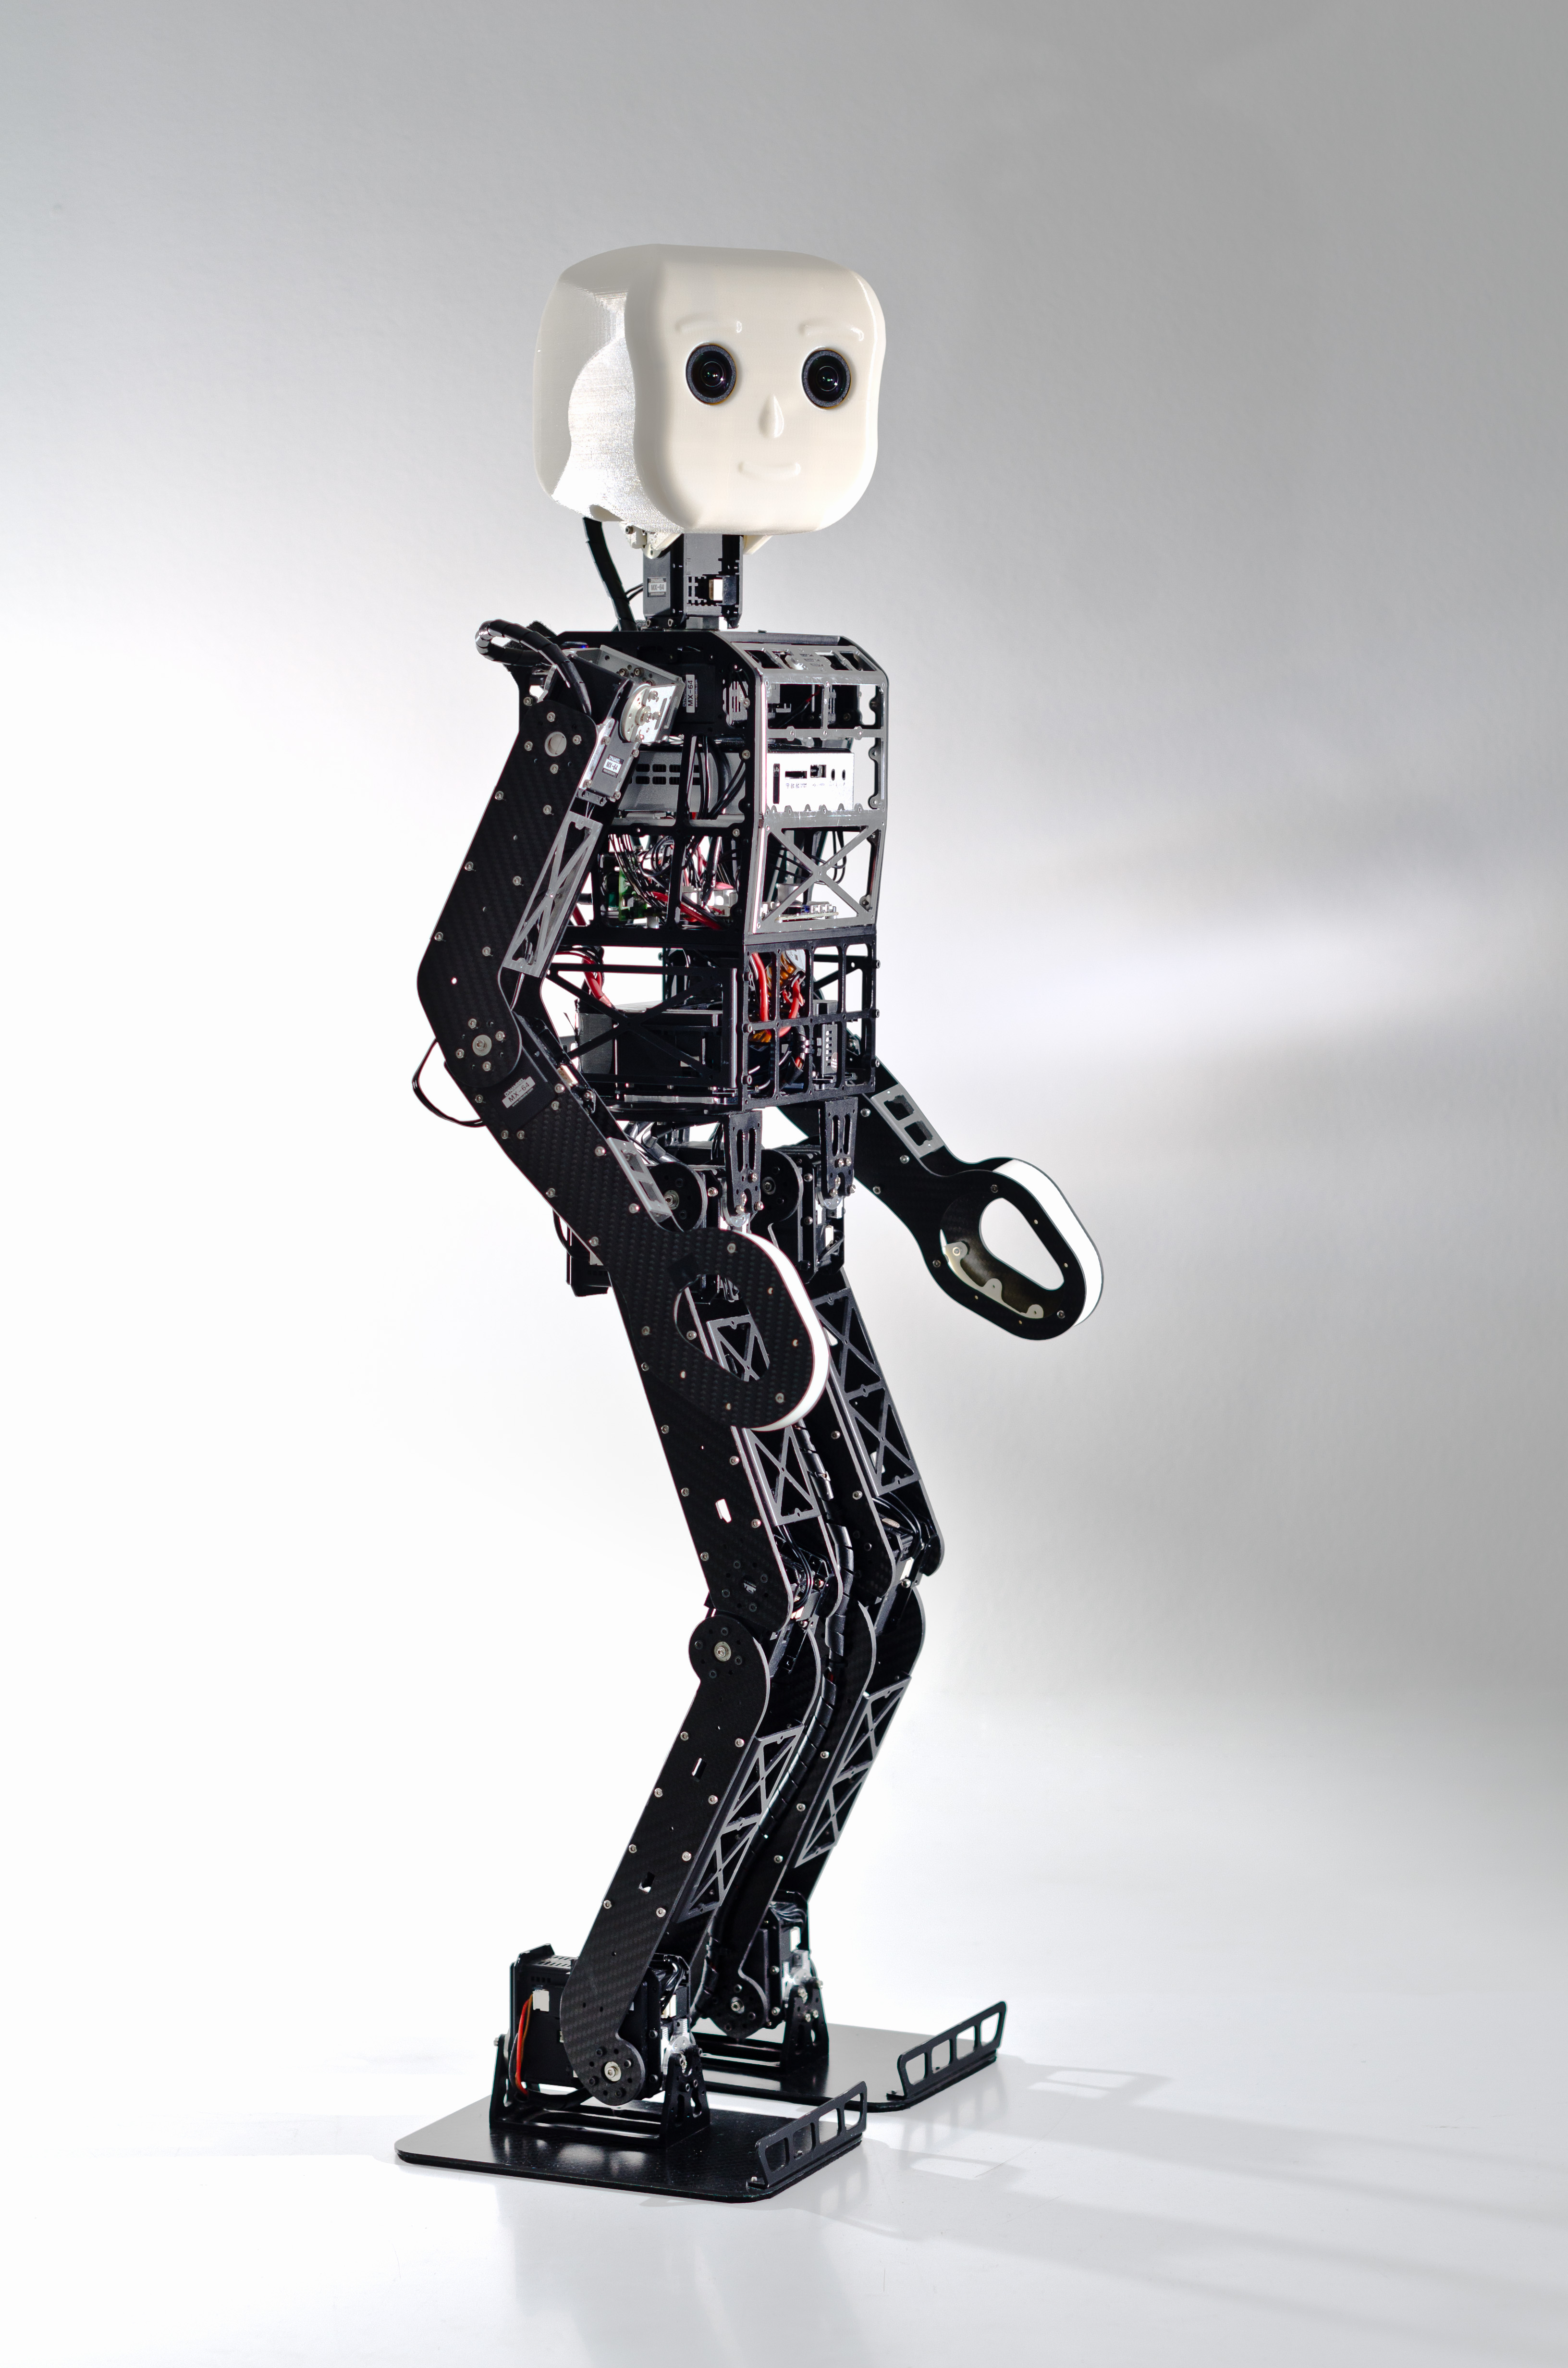
\includegraphics[height=6cm]{nimbro-op_1.jpg}}
    \hfil
    \subfloat[][]{\includegraphics[height=6cm]{nimbro-op_2.jpg}}
    \caption{Nimbro}
    \label{fig:nimbro_op_robot}
\end{figure}


\begin{figure}[]
\centering
    \subfloat[][]{\includegraphics[height=5.8cm]{icub_1.jpg}}
    \hfil
    \subfloat[][]{\includegraphics[height=5.8cm]{icub_2.jpg}}
    \caption{iCub is an open source humanoid robot developped by ITT(italy). Its cost is around \$300,000}
    \label{fig:icub_robot}
\end{figure}


\begin{figure}[]
\centering
    \subfloat[][Romela Thor]{\includegraphics[height=6cm]{thor_robot.png}}
    \hfil
    \subfloat[][Thor OP]{\includegraphics[height=6cm]{thor-op.jpg}}
    \hfil
    \subfloat[][zoom of the Thor structure]{\includegraphics[height=5cm]{zoom_thor.png}}
    \caption{Three humanoid robots made by KumoTek (USA).}
    \label{fig:kumotek_robots}
\end{figure}

\begin{figure}[]
    \begin{center}
        \includegraphics[height=6cm]{hrp2.jpg}
    \end{center}
    \caption{Kawada industry}
    \label{fig:hrp2_robot}
\end{figure}

\begin{figure}[]
    \begin{center}
        \includegraphics[height=6cm]{atlas_robot.jpg}
    \end{center}
    \caption{ATLAS}
    \label{fig:atlas_robot}
\end{figure}


\begin{figure}[]
    \begin{center}
        \includegraphics[height=6cm]{REEMC.jpg}
    \end{center}
    \caption{Reem C }
    \label{fig:reem_c_robot}
\end{figure}

\begin{figure}[]
    \begin{center}
        \includegraphics[width=0.8\linewidth]{hubo_robot_2.png}
    \end{center}
    \caption{Hubo II, KAIST}
    \label{fig:hubo_robot}
\end{figure}


\subsection{Laboratory prototypes} % (fold)

\begin{figure}[]
    \begin{center}
        \includegraphics[width=0.8\linewidth]{kenshiro.png}
    \end{center}
    \caption{Hubo II, KAIST}
    \label{fig:kenshiro_robot}
\end{figure}

\begin{figure}[]
    \begin{center}
        \includegraphics[width=0.8\linewidth]{cb2_robot.jpg}
    \end{center}
    \caption{CB2}
    \label{fig:cb2_robot}
\end{figure}

\begin{figure}[]
    \begin{center}
        \includegraphics[height=6cm]{biobiped.jpg}
    \end{center}
    \caption{Hubo II, KAIST}
    \label{fig:biobiped_robot}
\end{figure}


\begin{figure}[]
\centering
    \subfloat[][Denise]{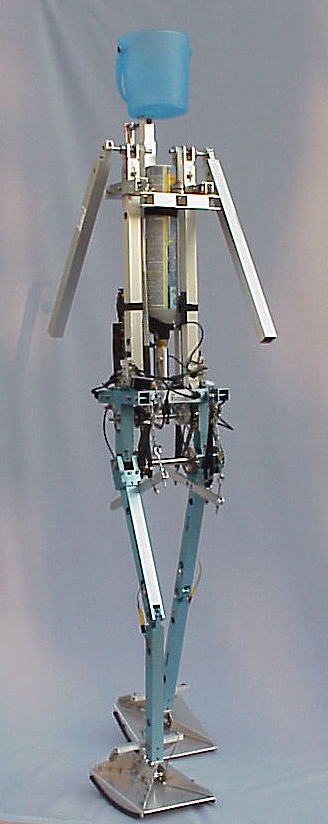
\includegraphics[height=6cm]{denise.jpg}}
    \hfil
    \subfloat[][Flame]{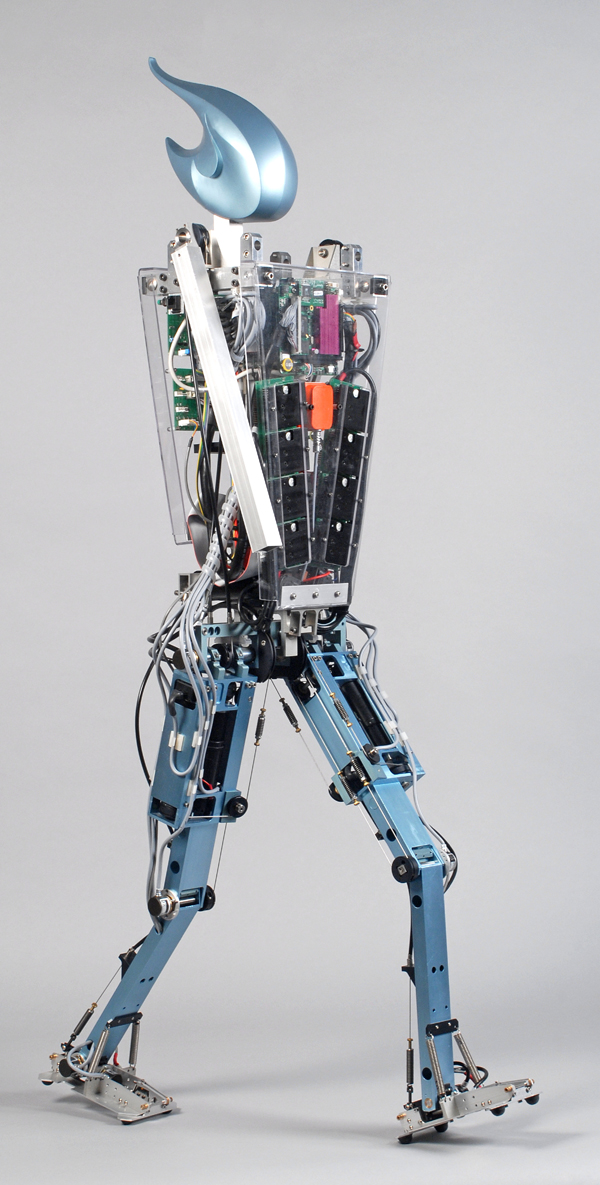
\includegraphics[height=6cm]{flame.jpg}}
    \hfil
    \subfloat[][Tulip]{\includegraphics[height=6cm]{tulip.jpg}}
    \caption{Three humanoid robots made by KumoTek (USA).}
    \label{fig:delft_passive_robots}
\end{figure}

\begin{figure}[]
    \begin{center}
        \includegraphics[height=6cm]{DLR-biped.jpg}
    \end{center}
    \caption{Hubo II, KAIST}
    \label{fig:DLR-robot}
\end{figure}

\begin{figure}[]
\centering
    \subfloat[][Acroban]{\includegraphics[height=6cm]{Acroban_1.jpg}}
    \hfil
    \subfloat[][Acroban]{\includegraphics[height=6cm]{Acroban_2.jpg}}
    \hfil
    \subfloat[][SigmaBan]{\includegraphics[height=6cm]{sigmaban.jpg}}
    \caption{Acroban}
    \label{fig:acroban_robot}
\end{figure}


\begin{figure}[]
    \begin{center}
        \includegraphics[height=6cm]{COMAN_robot.jpg}
    \end{center}
    \caption{COMAN ITT}
    \label{fig:coman-robot}
\end{figure}

\begin{figure}[]
\centering
    \subfloat[][Petman ?]{\includegraphics[height=6cm]{petman_proto.jpg}}
    \hfil
    \subfloat[][Petman]{\includegraphics[height=6cm]{petman.jpg}}
    \caption{Three humanoid robots made by KumoTek (USA).}
    \label{fig:petman_robot}
\end{figure}

DarwinOP c'est comme Poppy mais pas forcement pensé pour explorer le role du corps.

\subsubsection{Prototype} % (fold)

\subsection{Commercial} % (fold)

Aside the robot prototype,

Darwin \cite{ha2011development}

Other current research platforms are easily accessible and easy to use such as Nao \cite{gouaillier2008nao}, Darwin Op \cite{ha2011development}, Nimbro Op \cite{schwarznimbro} or iCub \cite{metta2008icub}.
Yet, they provide a "traditional" morphology (e.g.
limited compliance, rigid torso, big feet, over actuated) which can not be easily modified.
It makes them unadapted to study the impact of the morphology on biped locomotion and human physical interaction.

Each of these platforms provides key features for robotics but none of them regroups all the ones needed to explore both biped locomotion and physical interaction.

\section{methods for building robots} % (fold)
icub~\cite{tsagarakis2007icub}

\subsection{Actuation} % (fold)


\subsubsection{wire-driven} % (fold)

\subsubsection{Serie Elastic Actuator} % (fold)

\subsubsection{Pneumatic artificial muscle} % (fold)

\subsubsection{Hydraulic linear actuator} % (fold)


\section{Small humanoid robot} % (fold)
Research on humanoid robot is triving and had lead to a lot of humanoid robot.

We can cite Asimo has one of the first most advanced humanoid robot.

Despite this large number of humanoid platform only few reached a commercial distribution.
Among them there is only one adult sized robot, HRP2 while other are kid-size humanoid robot.

Darwin-OP was one of the first affordable and open source humanoid robot.
Based on the need in lab to have small  humanoid robot for research application.

For some reason, A 3D clone http://www.thingiverse.com/thing:9793
http://www.instructables.com/id/Robot-Cloning-by-DIY-3d-printers/
http://www.instructables.com/id/3D-Printed-Humanoid-Robot-for-under-100000-USD/

Darwin OP has not been really hacked.
Maybe it is due to the tools used.
SVN sucks, sourceforge is outdated.
The open community is more github centered


\section{Current limitations}

In the previous chapter, we presented several works showing the importance of the robot morphology and the need to continu the research in this domain.
However, we saw that none of the available commercial robot platform permits such scientific exploration.

Also, the current research practices in the Robotics field limit the diffusion and the impact of contributions.
Indeed, in most cases, there is no material associated with a published paper.
Meaning, only the theory is shared with the community but not the actual framework allowing to reproduce the results.

\begin{itemize}
    \item Lost of time, design a whole new robot.
    \item Morphology as an experimental variable
    \item Current robotic platforms do not permit to explore the morphology as a variable.
    \item IA haut niveau qui peut se faire en simulation avec certaines reserves.
    \item Currently, robot platform are not satisfying if we want to explore the role of morphology.
    They are not hackable and proto or not both easy to use and accessible.
    \item Problem with simulator VS real world
    \item Exploring control with real robot raise challenge due to error
    \item Morphologie as variable experimental
    \item Engineering on the platform not research
    \item There is two categories, commercial platform and research lab prototype.
    \item No distribution of the code
    \item no benchmark platform
    \item no hackable platform
\end{itemize}

This raises limitations for:
\begin{itemize}
    \item verifying the quality of the results presented in the paper,
    \item the reuse of the contribution as there is, in most case, a gap between the theory and the actual implementation,
    \item the collaborative work with other laboratory
\end{itemize}

However in the context of exploring control algorithm or studying the role of morphology, the actual robot is needed.
Also in this context, it raises major issue concerning the way to share material associated to a scientific contribution.

In this chapter, we present a design methodology allowing to:
\begin{itemize}
    \item consider the morphology as an experimental variable.
    \item easily share our results with the scientific community
\end{itemize}


\section{methods for dissemination and reproducibility} % (fold)

The most common way to  research

Share science

Currently most of the research dessiminatino is done through paper publications.
While papers are a high quality way to distribute the

Papers are good to present theoritical idea and results of experiment in high quality formated and writing way.
Yet, it is the descendent of the old way to share science coming from a time were Internet did not exist.

The scientific impact could be even more efficient with the use of web modern tools.

It is the intrinsic purpose of Internet to share between people.
The first purpose was even specific to the sharing of paper.
Twenty years later, the use of internet for scientific purpose does not really change while community driven project as shown amazing innovative works.

However, the research ranking is still only based on paper impact factor while using the modern tools can lead to a demultiplicaiton of this impact by dozens ...

Any obscure youtube video is more seen than the paper is read.

Optional works such has publishing code or videos is not encouraged by the current way to rank research.

However, a paper is a nice way to present theory but is not enough.
Most of our works are based on experiment results and only few paper actual share the experimental setup to reproduce the results.

While this can be counterproductive for the diffusion of the scientific works, it raise also probelm concerning the validation of experimental result and posibility to change parameter to evaluate the stability of a given algorithm.

Applying theoritical model presented in a paper on an actual experimental setup is really time consumming.

In case you didn’t know, academic publishing is undergoing a major upheaval.
Again.
It used to be that original discoveries could only be disseminated on paper, published in books and journals, which were mostly found in university libraries because their cost was so high.
Then the internet was invented and things began to change, but surprisingly slowly.
The big journals still ruled the roost—and even now they still really do, though future of this is uncertain—but paper and libraries eventually started to become less popular among readers.
Readers wanted their science to be indexed on the Web and they wanted instant PDF downloads.
Journals obliged and competed to add these features at no extra cost.
But you still needed a subscription to the journal—or your university library did—to get access to the article for less than \$30/article at the major journals.
This is still the typical state of affairs with most journals that predate the internet.

But then something new started happening: first online journals (never on paper) and then so-called open-access journals (online journals that were accessible to readers for free) started to pop up.
You may be surprised to learn that these journals are not much cheaper to produce than hardcopy magazines and books—despite the lack of paper—because most of the cost producing a journal is in the editorial services (copy editing, peer review, formatting, layout, marketing, etc).
Whereas online journals having the traditional subscription-for-access model charged the reader, open access models charged the authors.
Either way, a huge portion of the governmental science budget went towards paying for science publication, though funding agencies tended to prefer open access because the public could access the materials for free.

Novel journal are rising such as https://peerj.com/ which offer free reading and public review + the ability to ask question.

Non informal exchange between scientific.
Everyone is working in his lab and wait for the next conf to discuss with other people.
Forum man !

The scientific impact and dessimination could be way more efficient if modern tools was used.

Current research
publish paper ...

Some info on a website ...

le gars du LAAS qui donne une VM

emails

open source (soft)

Matlab Exchange

Science community

Hack your PhD


\textbf{object}: Review of the robot, in particular biped.


\textbf{Conclusion}: There is no adapted or replicable platform.
We need to create one.

